\documentclass[12pt,graphicx,caption,rotating]{article}
\textheight=24cm
\textwidth=18cm
\topmargin=-2cm
\oddsidemargin=0cm
\usepackage[utf8x]{inputenc}
\usepackage[activeacute,spanish]{babel}
\usepackage{graphicx}
\usepackage{times}
\usepackage{amssymb,amsfonts}
\usepackage[tbtags]{amsmath}
\usepackage{cite}
\usepackage{pict2e}
\usepackage{float}
\usepackage{lscape}
\usepackage[all]{xy}
\usepackage{graphics,graphicx,color,colortbl}
\usepackage{times}
\usepackage{subfigure}
\usepackage{wrapfig}
\usepackage{multicol}
\usepackage{cite}
\usepackage{url}
\usepackage[tbtags]{amsmath}
\usepackage{amsmath,amssymb,amsfonts,amsbsy}
\usepackage{listings}
\usepackage{bm}
%\usepackage{algorithm}
%\usepackage{algorithmic}
\usepackage[centerlast, small]{caption}
\usepackage[colorlinks=true, citecolor=blue, linkcolor=blue, urlcolor=blue, breaklinks=true]{hyperref}
\hyphenation{ele-men-tos he-rra-mi-en-ta cons-tru-yen trans-fe-ren-ci-a pro-pu-es-tas si-mu-lar vi-sua-li-za-cion}

\begin{document}
\title{Modulo de Potencia, Sensor y ADC}
\author{}
\date{}
\maketitle
%\markboth{Universidad Nacional de Colombia}{}
\floatname{algorithm}{Algoritmo}

\section{Modulo Potencia}
\noindent
Este modulo se encarga de determinar la intensidad lumínica que debe irradiar la fuente de luz, que para este caso es un bombillo incandescente de $60\, W$, el cual es graduado por medio de un potenciómetro.\\
Consta de un \textbf{Triac} o \textbf{Triodo para Corriente Alterna} \textbf{C106}\cite{c106} el cual se encarga de conmutar la corriente alterna, se usa para controlar el flujo de corriente promedio a una carga, con la particularidad de que conduce en ambos sentidos y puede ser bloqueado por inversión de la tensión.\\
También posee un \textbf{DIAC} o \textbf{Diodo de Disparo Bidireccional} \textbf{HT32}\cite{diac} diseñado para disparar el \textbf{Triac}, se comporta como $2$ diodos zener conectados en serie, pero orientados en formas opuestas.\\
Finalmente un \textbf{Potenciómetro} que es un resistor cuyo valor de resistencia es variable y permite controlar la intensidad lumínica del bombillo.\\
Para poder controlar la intensidad del bombillo con los componentes anteriores se utilizó el montaje de la Figura~\ref{fig1}.
\begin{figure}[H]
  \centering
    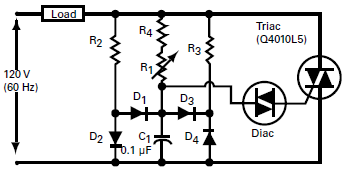
\includegraphics[scale=1]{Montaje_de_potencia.png}
      \caption{Montaje del Modulo de Potencia.}
	\label{fig1}
\end{figure}
\noindent
Para poder controlar el encendido y apagado del bombillo a determinadas horas fue necesario utilizar un relevo a $12\, V$ y un circuito integrado \textbf{ULN2803APG}\cite{uln} el cual se polariza a $12\, V$ tiene una entrada de $3.3\, V$ y una salida a $12\, V$, esto para poder utilizar una salida de la FPGA y poder encender el bombillo, es decir se utilizó como interruptor.

\subsection{Materiales Y Costos}
\begin{table}[H]
  \caption{Tabla de materiales y costos.}
  \centering
  \begin{tabular}{|c|c|r|c|r|}\hline
    \textbf{Elemento} & \textbf{Referencia} & \textbf{Valor Unitario} & \textbf{Cantidad} & \textbf{Total} \\ \hline
    \textbf{Conector} & $2$ entradas & $300$ & \textbf{3} & $900$ \\ \hline
    \textbf{Diodos} & $1n4004$ & $200$ & \textbf{4} & $800$ \\ \hline
    \multicolumn{ 1}{|c|}{\textbf{Resistencias}} & $15\, K\Omega$ & $100$ & \textbf{2} & $200$ \\ \cline{ 2- 5}
    \textbf{} & $4.9\, K\Omega$ & $100$ & \textbf{2} & $200$ \\ \hline
    \textbf{Potenciómetro} & $1\, M\Omega$ & $800$ & \textbf{3} & $2400$ \\ \hline
    \textbf{Condensador} & $0.1\, \mu F$ & $100$ & \textbf{1} & $100$ \\ \hline
    \textbf{Regulador} & $ULN2803APG$ & $1500$ & \textbf{1} & $1500$ \\ \hline
    \textbf{Relevo} & $12\, V$ a $1\, A$ & $2000$ & \textbf{1} & $2000$ \\ \hline
    \textbf{DIAC} & $HT32$ & $300$ & \textbf{3} & $900$ \\ \hline
    \textbf{TRIAC} & $C106$ & $1600$ & \textbf{3} & $4800$ \\ \hline
    \multicolumn{ 4}{|c|}{\textbf{Total}} & \textbf{13800} \\ \cline{ 5- 5}\hline
   \end{tabular}
   \label{tab1}
\end{table}

\subsection{Dificultades}
\begin{itemize}
 \item Uno de los problemas más grandes que se tuvieron fue al momento de soldar tanto el TRIAC como el DIAC, con el empaque que tienen no pueden soportar por mucho tiempo la temperatura generada por el cautin.
 \item El realizar el interruptor por medio del relevo y del $ULN2803APG$ determinando los tiempos de encendido y pagado que se habían programado en la FPGA, esa sincronización no se pudo realizar por falta de tiempo.
\end{itemize}

\section{Sensor y ADC}
\noindent
Para la etapa de adquisición de datos se utilizo el sensor \textbf{GA1A2S100SS}\cite{sensor} que funciona de manera óptima en una polarización de $3\, V$ y da un rango de $100\, mV$ este rango se dio cuando se ilumino con luz ambiente hasta máxima intensidad de luz producida por el bombillo.\\
Como la FPGA no tiene una entrada análoga fue necesario utilizar un conversor análogo-digital el \textbf{ADC0804}\cite{adc}, este ADC tiene una salida paralela de $8\, bits$, para esta etapa se utilizaron en realidad $6\, bits$ los cuales se envían para la parte de visualización. Se utilizaron los montajes sugeridos por \cite{sensor}, el cual se muestra en la Figura~\ref{fig2}.
\begin{figure}[H]
  \centering
    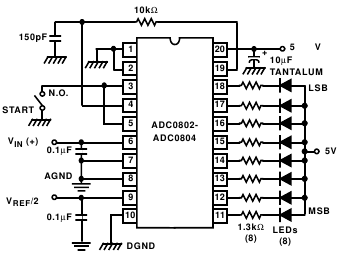
\includegraphics[scale=0.7]{adc.png}
      \caption{Montaje para el ADC.\cite{adc} (Página $16$)}
	\label{fig2}
\end{figure}

\subsection{Materiales Y Costos}
\begin{table}[H]
  \caption{Tabla de materiales y costos.}
  \centering
  \begin{tabular}{|c|c|r|c|r|}\hline
    \textbf{Elemento} & \textbf{Referencia} & \textbf{Valor Unitario} & \textbf{Cantidad} & \textbf{Total} \\ \hline
    \textbf{Regleta} & $40$ entradas & $900$ & \textbf{1} & $900$ \\ \hline
    \textbf{LED} & $LED$ & $200$ & \textbf{10} & $2000$ \\ \hline
    \textbf{} & $10\, K\Omega$ & $100$ & \textbf{2} & $200$ \\ \cline{ 2- 5}
    \textbf{} & $2\, K\Omega$ & $100$ & \textbf{2} & $200$ \\ \cline{ 2- 5}
    \multicolumn{ 1}{|c|}{\textbf{Resistencias}} & $3\, K\Omega$ & $100$ & \textbf{2} & $200$ \\ \cline{ 2- 5}
    \textbf{} & $5.8\, K\Omega$ & $100$ & \textbf{2} & $200$ \\ \cline{ 2- 5}
    \textbf{} & $3.3\, K\Omega$ & $100$ & \textbf{2} & $200$ \\ \hline
    \textbf{Ribon} & $10$ hilos & $1000$ & \textbf{1} & $1000$ \\ \hline
    \textbf{Conector Ribon} & $10$ entradas & $1000$ & \textbf{1} & $1000$ \\ \hline
    \textbf{Sensor} & $GA1A2S100SS$ & $3700$ & \textbf{1} & $3700$ \\ \hline
    \textbf{ADC} & $ADC0804$ & $8700$ & \textbf{1} & $8700$ \\ \hline
    \multicolumn{ 4}{|c|}{\textbf{Total}} & \textbf{18300} \\ \cline{ 5- 5}\hline
   \end{tabular}
   \label{tab2}
\end{table}

\subsection{Dificultades}
\begin{itemize}
 \item Para esta fue muy complicado caracterizar el $ADC0804$ especialmente el $V_{REF/2}$, como no se sabia cual era el mejor voltaje de polarización al inicio fue muy complicado observar las variaciones que mostraba el ADC.
 \item El modulo que se desarrollo en la FPGA fue difícil de sincronizar por la falta de tiempo para poder determinar los valores de variación. Este modulo se trato de implementar pero fallo por la falta del modulo principal de visualización, no hubo suficiente tiempo para sincronizar la parte análoga con la parte digital.
\end{itemize}


\bibliographystyle{ieeetran}
\begin{thebibliography}{99}
  \bibitem{uln} Sitio Web \url{http://www.semicon.toshiba.co.jp/info/docget.jsp?pid=ULN2803APG&lang=en&type=datasheet}.
  
  \bibitem{c106} Sitio Web \url{http://www.onsemi.com/pub_link/Collateral/C106-D.PDF}.
  
  \bibitem{diac} Sitio Web \url{http://pdf.datasheetcatalog.com/datasheets/560/170346_DS.pdf}.
  
  \bibitem{sensor} Sitio Web \url{http://www.sigmaelectronica.net/manuals/GA1A2S100SS.pdf}.
  
  \bibitem{adc} Sitio Web \url{http://www.sigmaelectronica.net/manuals/ADC0804.pdf}
\end{thebibliography}
\end{document}